\documentclass[tikz,border=3pt]{standalone}
\usepackage{amsmath}
\usetikzlibrary{arrows.meta,positioning,fit,calc,backgrounds}
\definecolor{ink}{HTML}{1F2933}
\definecolor{muted}{HTML}{667085}
\definecolor{blue}{HTML}{2563EB}
\definecolor{teal}{HTML}{0F766E}
\definecolor{green}{HTML}{15803D}
\definecolor{amber}{HTML}{B7791F}
\definecolor{red}{HTML}{B91C1C}
\definecolor{gray}{HTML}{6B7280}
\tikzset{
  block/.style={draw=#1, rounded corners=1.8pt, line width=0.55pt, fill=white, minimum width=26mm, minimum height=8.5mm, align=center, font=\scriptsize},
  tag/.style={draw=#1, rounded corners=1.2pt, line width=0.45pt, fill=#1!7, inner xsep=2pt, inner ysep=1pt, font=\tiny},
  lane/.style={draw=#1!45, fill=#1!4, rounded corners=2pt, inner sep=3pt},
  arr/.style={-{Latex[length=1.7mm]}, line width=0.55pt, draw=ink}
}
\begin{document}
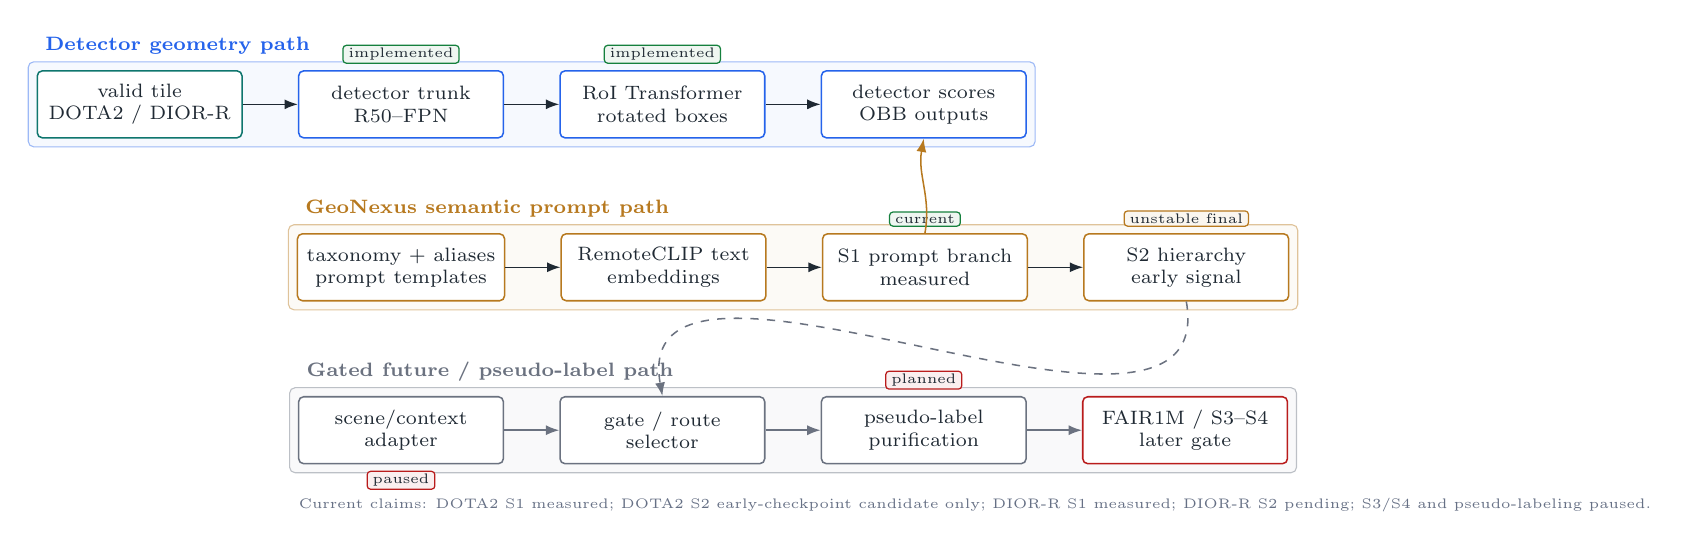
\begin{tikzpicture}[font=\sffamily, text=ink, node distance=7mm]
  \node[block=teal] (tile) {valid tile\\DOTA2 / DIOR-R};
  \node[block=blue, right=of tile] (fpn) {detector trunk\\R50--FPN};
  \node[block=blue, right=of fpn] (roi) {RoI Transformer\\rotated boxes};
  \node[block=blue, right=of roi] (scores) {detector scores\\OBB outputs};
  \node[tag=green, above=0.8mm of fpn] {implemented};
  \node[tag=green, above=0.8mm of roi] {implemented};
  \draw[arr] (tile) -- (fpn);
  \draw[arr] (fpn) -- (roi);
  \draw[arr] (roi) -- (scores);
  \begin{scope}[on background layer]
    \node[lane=blue, fit=(tile)(fpn)(roi)(scores)] (laneA) {};
  \end{scope}
  \node[anchor=west, font=\scriptsize\bfseries, text=blue] at ($(laneA.north west)+(1mm,2mm)$) {Detector geometry path};

  \node[block=amber, below=12mm of fpn] (tax) {taxonomy + aliases\\prompt templates};
  \node[block=amber, right=of tax] (clip) {RemoteCLIP text\\embeddings};
  \node[block=amber, right=of clip] (s1) {S1 prompt branch\\measured};
  \node[block=amber, right=of s1] (s2) {S2 hierarchy\\early signal};
  \node[tag=green, above=0.8mm of s1] {current};
  \node[tag=amber, above=0.8mm of s2] {unstable final};
  \draw[arr] (tax) -- (clip);
  \draw[arr] (clip) -- (s1);
  \draw[arr] (s1) -- (s2);
  \draw[arr, draw=amber] (s1.north) to[out=80,in=-100] (scores.south);
  \begin{scope}[on background layer]
    \node[lane=amber, fit=(tax)(clip)(s1)(s2)] (laneB) {};
  \end{scope}
  \node[anchor=west, font=\scriptsize\bfseries, text=amber] at ($(laneB.north west)+(1mm,2mm)$) {GeoNexus semantic prompt path};

  \node[block=gray, below=12mm of tax] (ctx) {scene/context\\adapter};
  \node[block=gray, right=of ctx] (gate) {gate / route\\selector};
  \node[block=gray, right=of gate] (pseudo) {pseudo-label\\purification};
  \node[block=red, right=of pseudo] (fair) {FAIR1M / S3--S4\\later gate};
  \node[tag=red, below=0.8mm of ctx] {paused};
  \node[tag=red, above=0.8mm of pseudo] {planned};
  \draw[arr, draw=gray] (ctx) -- (gate);
  \draw[arr, draw=gray] (gate) -- (pseudo);
  \draw[arr, draw=gray] (pseudo) -- (fair);
  \draw[arr, draw=gray, dashed] (s2.south) to[out=-80,in=100] (gate.north);
  \begin{scope}[on background layer]
    \node[lane=gray, fit=(ctx)(gate)(pseudo)(fair)] (laneC) {};
  \end{scope}
  \node[anchor=west, font=\scriptsize\bfseries, text=gray] at ($(laneC.north west)+(1mm,2mm)$) {Gated future / pseudo-label path};

  \node[anchor=west, font=\tiny, text=muted] at ($(laneC.south west)+(0,-4mm)$)
  {Current claims: DOTA2 S1 measured; DOTA2 S2 early-checkpoint candidate only; DIOR-R S1 measured; DIOR-R S2 pending; S3/S4 and pseudo-labeling paused.};
\end{tikzpicture}
\end{document}
